\documentclass[12pt,a4paper]{article}
 
%encoding
%--------------------------------------
\usepackage[utf8]{inputenc}
\usepackage[T1]{fontenc}
%--------------------------------------
 
%Portuguese-specific commands
%--------------------------------------
\usepackage[portuguese]{babel}
%--------------------------------------
 
%Hyphenation rules
%--------------------------------------
\usepackage{hyphenat}
\hyphenation{mate-mática recu-perar}
%--------------------------------------

\usepackage{graphicx}
\graphicspath{ {images/} }
\usepackage{caption}
\usepackage{subcaption}
\usepackage{amsmath}

\begin{document}

\begin{titlepage}
\centering
{\LARGE Instituto Superior de Engenharia de Lisboa \par}
\vspace{1cm}
{\Large Codificação de Sinais Multimédia\par}
{\Large 2º Semestre 2016/2017\par}
\vspace{1.5cm}
{\huge 1º Trabalho prático\par}
\vspace{2cm}
{\Large João Santos nº 39348\par}
\end{titlepage}

\tableofcontents
\listoffigures

\clearpage

\section{Introdução}
O primeiro trabalho prático da disciplina de Codificação de Sinais Multimédia tem como objetivo a utilização da biblioteca OpenCV (Open Source Computer Vision Library) para processamento de imagens através da linguagem Python. Através da utilização desta biblioteca é pretendido realizar operações em imagens, tais como, alterações de qualidade de imagens, conversões de imagens para níveis de cinzento e operações morfológicas com valores de pixeis. O primeiro trabalho prático serve como ambientação há biblioteca OpenCV pois esta biblioteca irá ser utilizada nos próximos trabalhos práticos.

\clearpage

\section{Desenvolvimento}
Este trabalho prático tem como fio de desenvolvimento sete questões que devem ser respondidas e os seus resultados analisados. Seis das questões presentes no enunciado do trabalho são referentes à imagem de referência "\textit{Lena}", imagem essa que pode ser observada na figura 1.

\begin{figure}[h]
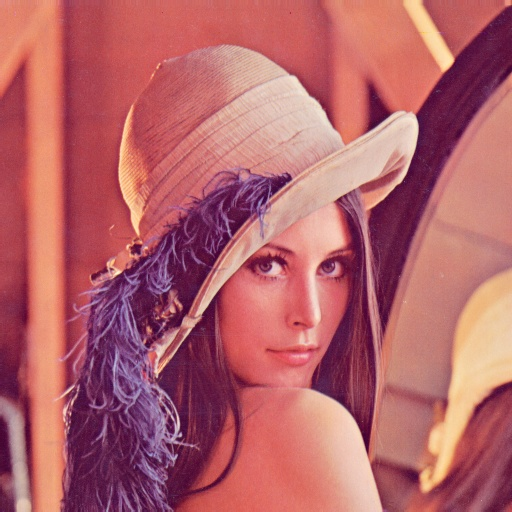
\includegraphics[scale=0.5]{lenacc}
\centering
\caption{Imagem original "Lena".}
\end{figure}

Tendo em conta o referido anteriormente iremos agora delinear cada um dos pontos apresentados no enunciado e as respetivas resoluções.

\clearpage

\subsection{Imagem original}
De modo a implementar o esperado foi utilizada a biblioteca OpenCV, mais especificamente o método imread("pathname"). O código implementado, tal como, apresentado no enunciado foi o seguinte:\\
\newline
lena = cv2.imread("images/lenac.tif")\\
cv2.imshow("Lena original", lena)\\
print "dtype: ", lena.dtype\\
print "shape: ", lena.shape\\
\newline
Observando os resultados da execução do código observou-se que a imagem resultado do imshow() é igual à figura 1 e os resultados do "dtype" e "shape" foram os seguintes:\\
\newline
dtype: uint8\\
shape: (512,512,3)\\
\newline
O campo dtype = uint8 tem como significado a quantidade de bits utilizada para realizar a codificação da imagem, neste caso 8 bits para cada pixel.\\
Por sua vez o campo shape = (512,512,3) representa a dimensão da imagem, ou seja, 512x512 e o número 3 representa os planos de cor utilizado, neste caso, RGB.

\subsection{Tamanhos dos ficheiros, taxas de compressão, SNR e PSNR}
De modo a responder à segunda questão do enunciado foram implementadas as seguintes linhas de código:\\
\newline
cv2.imwrite('images/lena - 80\%.jpg', lena, (cv2.IMWRITE\_JPEG\_QUALITY,80))\\
cv2.imwrite('images/lena - 10\%.jpg', lena, (cv2.IMWRITE\_JPEG\_QUALITY,10))\\
\newline
Estas duas linhas de código permitem transformar a imagem original "lenac.tif" para uma imagem com qualidade de 80\% e 10\% no formato JPEG. De seguida foram efetuados prints dos tamanhos das imagens e observados os resultados.\\
\newline
\newline
Tamanho da imagem original: 786814\\
Tamanho da imagem com 80\% de qualidade: 44196\\
Tamanho da imagem com 10\% de qualidade: 9558\\
\newline
Observando os valores obtidos é intuitivo que reduzindo a qualidade da imagem reduzimos também o tamanho do seu ficheiro, isto porque, a quantidade de bits utilizada para codificar a imagem irá ser menor, dai o tamanho do ficheiro ser menor.\\
\newline
É possível observar através das figuras 2 e 3 as imagens com qualidades de 80\% e 10\%, respetivamente: 

\begin{figure}[h]
\centering
\begin{minipage}{.5\textwidth}
  \centering
  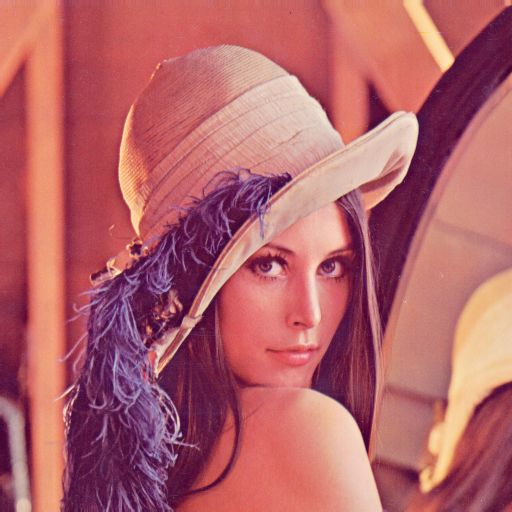
\includegraphics[scale=0.3]{lena80}
  \captionof{figure}{Qualidade de 80\%.}
\end{minipage}%
\begin{minipage}{.5\textwidth}
  \centering
  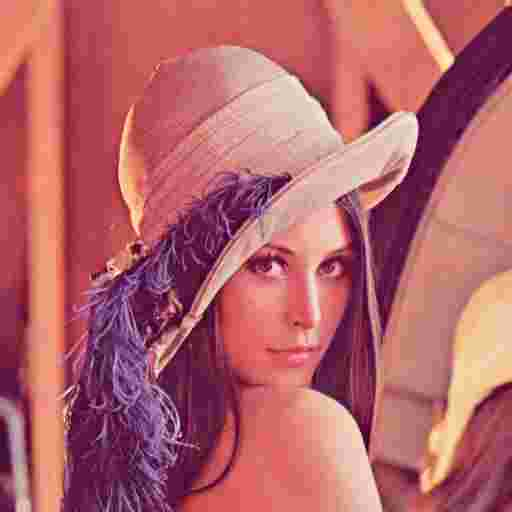
\includegraphics[scale=0.3]{lena10}
  \captionof{figure}{Qualidade de 10\%.}
\end{minipage}
\end{figure}

Obtendo ambas as imagens com qualidades diferentes foram calculadas as Taxas de Compressão, SNR e PNSR.\\\begin{itemize}
\item {Taxa de Compressão}
\end{itemize}
A Taxa de Compressão é uma medida de desempenho que é obtida através da razão entre o tamanho da imagem original e o tamanho da imagem após compressão. Uma Taxa de Compressão com valores menores significa que a imagem comprimida tem dimensão aproximada da imagem original, ou seja, não existiu uma compressão acentuada.\\
\[
\text{Taxa de compressão} = \frac{\text{Tamanho da imagem original}}{\text{Tamanho da imagem comprimida}}
\]
\newline
Calculando as Taxas de Compressão para as qualidades de 80\% e 10\%, respetivamente, foram obtidos os seguintes resultados:\\
\newline
Taxa de Compressão de uma imagem com 80\% de qualidade : 2.44\\
Taxa de Compressão de uma imagem com 10\% de qualidade: 11.27\\
\newline
Tendo em conta o que foi explicado anteriormente podemos observar que como a primeira imagem tem uma qualidade de 80\% a sua Taxa de Compressão irá tomar uma valor menor que a imagem com qualidade de 10\%.\\
\begin{itemize}
\item {SNR (Sinal-to-Noise Ratio)}
\end{itemize}
Seguidamente, foram efetuados os cálculos da SNR(Signal-to-noise ratio). Como o nome indica, a relação sinal-ruído é definida como a razão da potência de um sinal e a potência do ruído sobreposto ao sinal, ou seja, quanto maior o valor da SNR melhor será a relação entre a qualidade da imagem original e da imagem comprimida. O cálculo da SNR é efetuado utilizando a seguinte fórmula:\\
\newline
\[
SNR = 10\: log_{10}\: \frac{Psinal}{Pruido}
\]\\
\newline
Calculando as SNR's para as qualidades de 80\% e 10\%, respetivamente, foram obtidos os seguintes resultados:\\
\newline
SNR de uma imagem com 80\% de qualidade: 30.9\\
SNR de uma imagem com 10\% de qualidade: 22.87\\
\newline
Como esperado o valor da relação sinal-ruído irá ter uma valor mais elevado para a imagem com uma qualidade mais aproximada da imagem original.\\
\begin{itemize}
\item {PSNR (Peak Sinal-to-Noise Ratio)}
\end{itemize}
Finalmente foram efetuados os cálculos da PSNR (Peak Sinal-to-Noise Ratio), a PSNR é um termo utilizado para definir a relação entre a energia máxima de um sinal e o ruído que afeta a sua compressão. A PSNR é mais facilmente definida utilizando o MSE (Mean Squared Error), para tal, foram utilizadas as seguintes expressões matemáticas.\\
\newline
\[
MSE = \frac{1}{mn}\sum_{i=0}^{m-1}\sum_{j=0}^{n-1}\left [ I(i,j) - K(i,j)  \right]^2
\]\\
O MSE é definido utilizando uma imagem monocromática $I$ $m\times n$ sem ruído e uma imagem $K$ com ruído.
\[
PSNR = 20\: log_{10}(MAX_I) - 10\: log_{10}(MSE)
\]
Observando a expressão da PSNR o valor de $MAX_I$ representa o valor máximo de pixel na imagem, ou seja, quando os pixeis são representados usando 8 bits, o valor máximo é 255. Utilizando ambas as expressões os valores obtidos foram os seguintes:\\
\newline
PSNR com qualidade de imagem de 80\%: 31.27\\
PSNR com qualidade de imagem de 10\%: 23.24\\
\newline
O valores típicos de PSNR para imagem com compressão lossy utilizando 8 bits de codificação estão entre 30 e 50 dB, logo, podemos considerar que os nossos valores de PSNR se encontram dentro do esperado.

\subsection{Imagem em níveis de cinzento}
O terceiro objetivo do trabalho tem como objetivo a conversão da imagem original para uma em níveis de cinzento. A conversão para níveis de cinzento é efetuado utilizando o seguinte método do OpenCV:\\
\newline
lenaGray = cv2.cvtColor(lena , cv2.COLOR\_BGR2GRAY)\\
\newline
A utilização deste método implementa a expressão $Y = R\times 299/1000 + G\times 587/1000 + B\times 114/1000$, sendo que, o RGB corresponde a cada componente de cor RED, GREEN e BLUE. A expressão foi obtida devido ao facto da visão humana ser mais sensível ao verde e menos sensível ao azul, adiciona-se então 30\% do vermelho mais 59\% do verde e apenas 11\% do azul. Aplicando esta transformação a imagem obtida pode ser observada na figura 4.

\clearpage

\begin{figure}
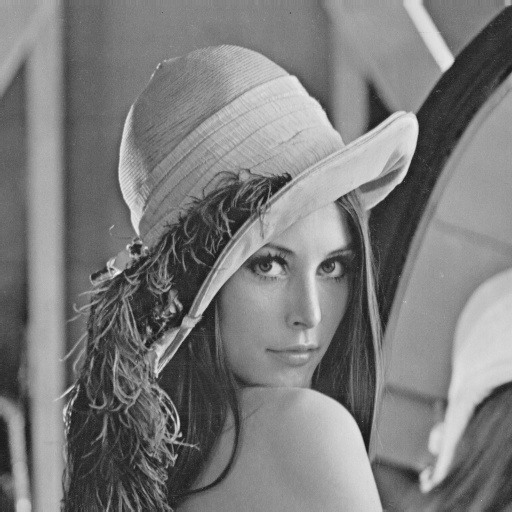
\includegraphics[scale=0.5]{lenaCinzento}
\centering
\caption{Imagem em tons de cinzento.}
\end{figure}

Posteriormente à transformação da imagem foi obtido o tamanho do ficheiro da mesma e comparado com o tamanho da imagem original, deste modo, os resultados obtidos foram os seguintes:\\
\newline
Tamanho da imagem original: 786814\\
Tamanho da imagem em níveis de cinzento: 91229\\
\newline
Observando os valores obtidos e a transformação aplicada é compreensível que o tamanho da imagem em níveis de cinzento irá ser menor que o da imagem original pois são necessários muito menos bits para a codificação da mesma.
\clearpage

\subsection{Histograma da imagem em níveis de cinzento}
O quarto ponto do trabalho requer a apresentação do histograma da imagem em tons de cinzento, para tal, foi utilizado o seguinte método da biblioteca matplotlib:\\
\newline
plt.hist(lenaGray.ravel(), 256, [0,256], normed = 1, facecolor = 'red')\\
\newline
Implementada a linha de código apresentada em cima o histograma obtido pode ser observado na figura 5.
\begin{figure}[h]
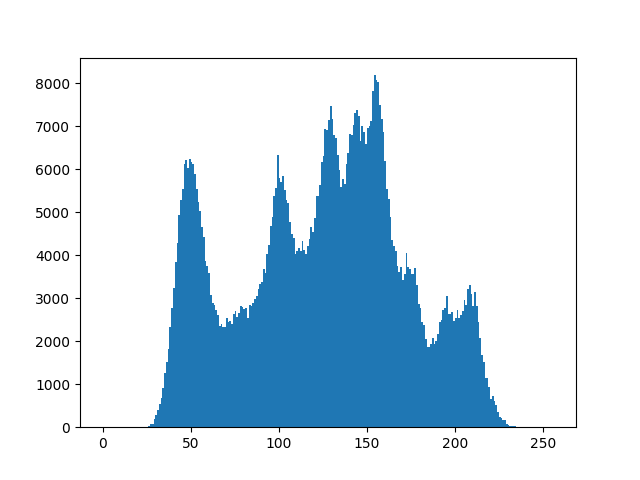
\includegraphics[scale=0.5]{histograma}
\centering
\caption{Histograma.}
\end{figure}

O histograma representa no eixo do $x$ o número de níveis de cinzento e no eiro dos $y$ o número de ocorrências de cada nível. É possível determinar a olho "nu" que não existem pixeis com o valor 0 (preto), nem pixeis com o valor 255 (branco). De maneira a contabilizar o número de níveis de cinzento foi utilizado o método da biblioteca numpy np.unique(lenaGray).size, este método retorna um array com todos os valores existentes sem repetições, ou seja, o comprimento desse array irá ser o número de níveis de cinzento existentes na imagem. É necessário ter em consideração que o valor 0 não é um nível de cinzento, logo, se existisse uma ocorrência desse valor esta tinha que ser retirada, assim o valor obtido de níveis de cinzento foi 215.

\subsection{Manipulação de pixeis na imagem}
No quinto ponto do trabalho é necessário realizar manipulação de pixeis. Existem pixeis com maior ou menor peso, ou seja, se considerarmos que o bit de maior peso é o $2^7 = 128$, isto permite que grande parte da informação seja mantida, ao contrario de um bit de menor peso que, como veremos mais à frente, a imagem fica impercetível. A manipulação de pixeis pode ser realiza através de shifts ou intersecções lógicas, deste modo é possível implementar a operação lenaGray \& 180 para obter o pixel mais significante da imagem. É possível representar os restantes pixeis menos significantes realizando interseções  lógicas usando os bits de menor peso. Um exemplo desta manipulação pode ser o seguinte, o primeiro bit da imagem tem um valor de 160, ou, 10100000 em binário. Realizando uma interceção lógico com o valor 100000000 (128) resulta o valor 128. Deste modo podemos observar que ainda se manteve parte da informação inicial. Caso a operação fosse realizada entre o valor 160 e o valor 16 (00010000) o resultado seria 0 (00000000), logo não ia existir nenhum bit ativo nesse pixels. A figura 6 representa os bits, $2^7, 2^6, 2^5, 2^4, 2^3, 2^2, 2^1$ e $2^0$, respetivamente.

\clearpage

\begin{figure}[h] 
\centering
  \begin{minipage}{0.4\linewidth}
    \centering
    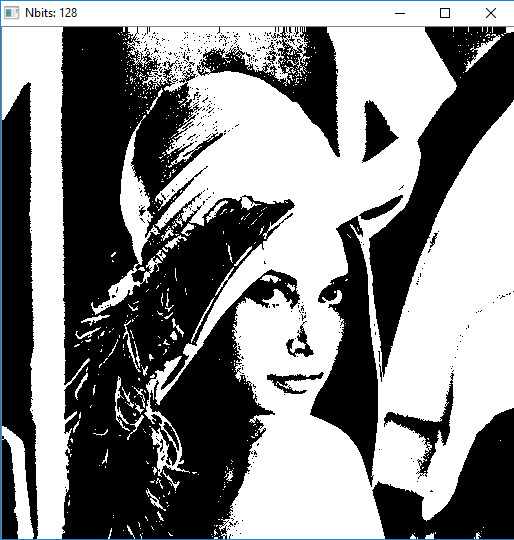
\includegraphics[width=.6\linewidth]{128} 
  \end{minipage}
  \begin{minipage}{0.4\linewidth}
    \centering
    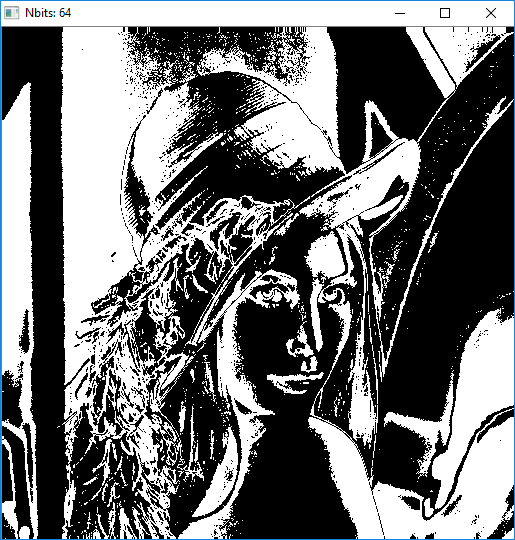
\includegraphics[width=.6\linewidth]{64} 
  \end{minipage} 
  \begin{minipage}{0.4\linewidth}
    \centering
    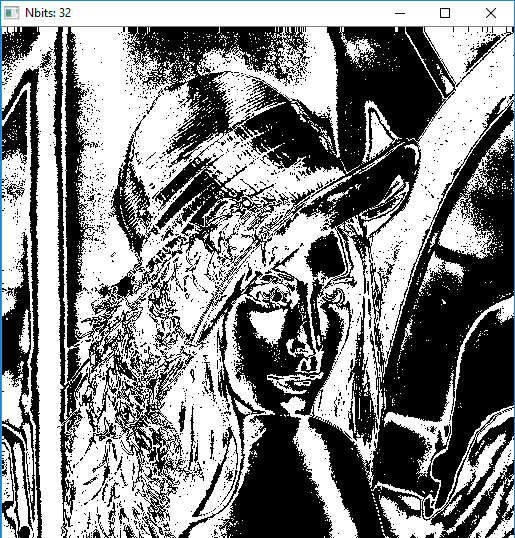
\includegraphics[width=.6\linewidth]{32} 
  \end{minipage} 
  \begin{minipage}{0.4\linewidth}
    \centering
    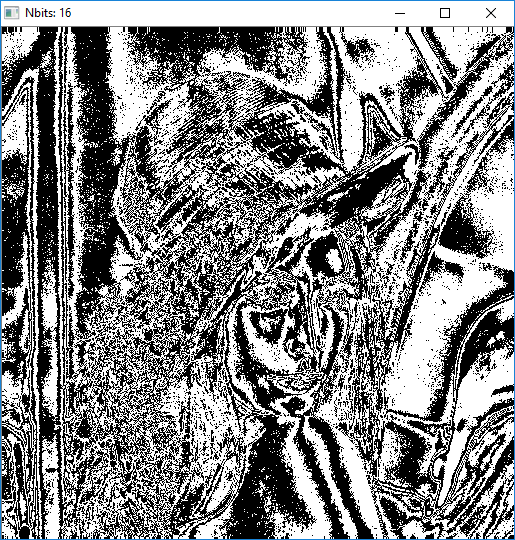
\includegraphics[width=.6\linewidth]{16} 
  \end{minipage}
  \begin{minipage}{0.4\linewidth}
    \centering
    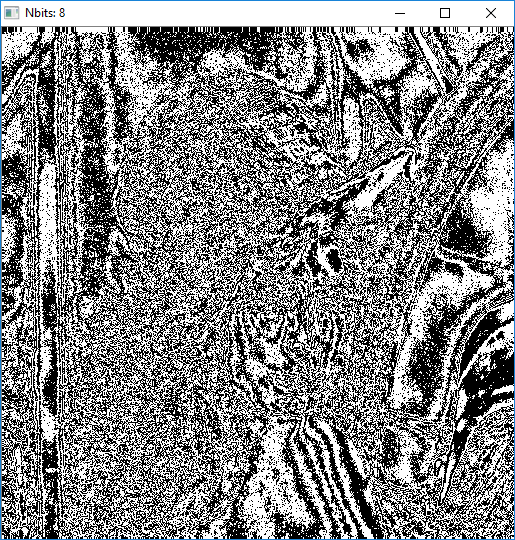
\includegraphics[width=.6\linewidth]{8} 
  \end{minipage}
  \begin{minipage}{0.4\linewidth}
    \centering
    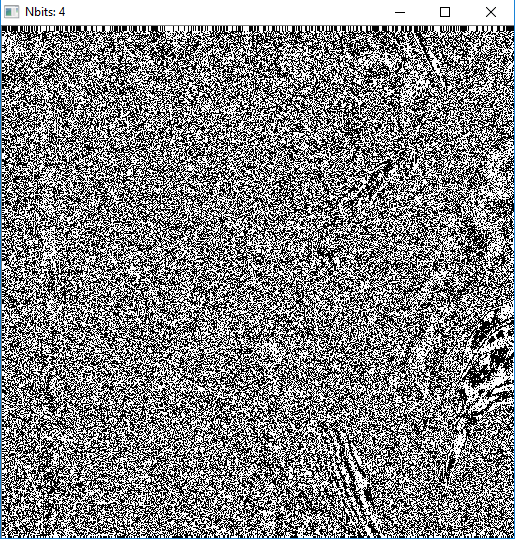
\includegraphics[width=.6\linewidth]{4} 
  \end{minipage} 
  \begin{minipage}{0.4\linewidth}
    \centering
    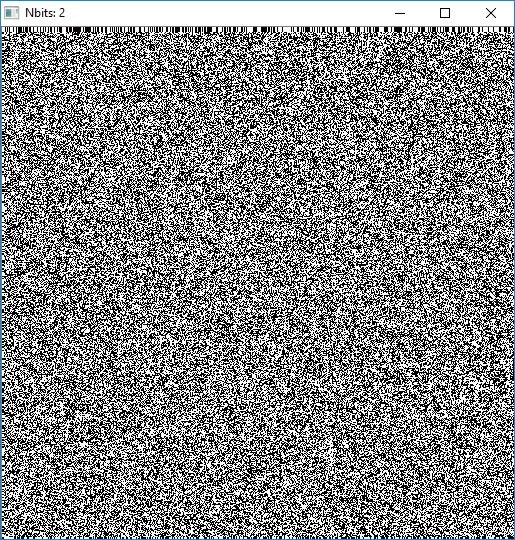
\includegraphics[width=.6\linewidth]{2} 
  \end{minipage} 
  \begin{minipage}{0.4\linewidth}
    \centering
    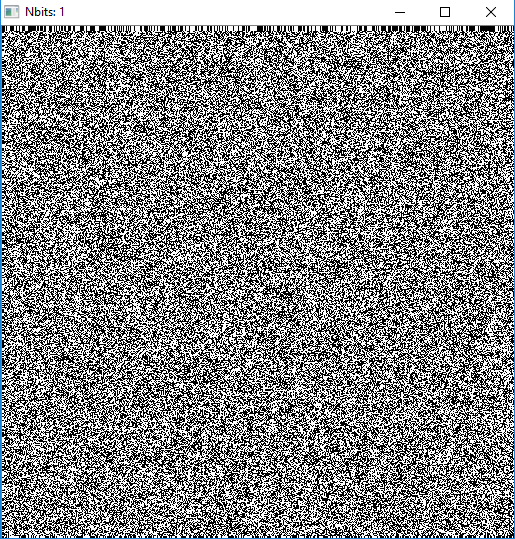
\includegraphics[width=.6\linewidth]{0} 
  \end{minipage}
  \caption{Imagens com a respetiva manipulação de bits.}
\end{figure}
\subsection{Manipulação dos quatro bits mais significantes da imagem}
A questão 6 do trabalho prático ainda vem salientar mais o que foi explicado no ponto anterior, ou seja, desta vez realizamos a operação de interseção utilizando os quatro bits mais significantes e observamos que a imagem obtida é visivelmente semelhante à imagem original. Utilizando o mesmo exemplo do ponto anterior mas desta vez com os quatro bits mais significantes obtemos o seguinte $\frac{10100000}{11110000}\& = 10100000 = 160$. O valor resultante da operação foi o mesmo valor inicial do pixel, ou seja, toda a informação foi mantida. Observado a  figura 7 e 8 a comparação da imagem original e da imagem com os quatro bits mais significantes.

\begin{figure}[h]
\centering
\begin{minipage}{.5\textwidth}
  \centering
  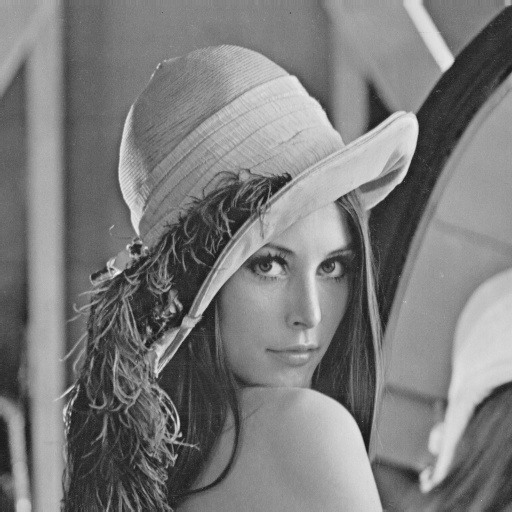
\includegraphics[scale=0.3]{lenaCinzento}
  \captionof{figure}{Imagem original.}
\end{minipage}%
\begin{minipage}{.5\textwidth}
  \centering
  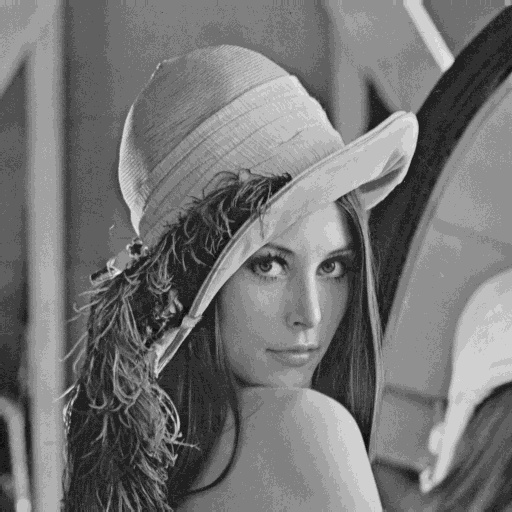
\includegraphics[scale=0.3]{quatrobits}
  \captionof{figure}{Imagem alterada.}
\end{minipage}
\end{figure}
Comparando as duas imagem é possível concluir que utilizando apenas os quatro bits mais significantes a imagem fica percetível e muito aproximada da imagem original.

\clearpage

\section{Conclusões}
Com a finalização do trabalho foram obtidos conhecimentos de métodos da biblioteca OpenCV que vão ser úteis nos trabalhos seguintes. A manipulação de bits de imagens binárias(ou outro tipo de média) é algo que vai ser essencial para a codificação e descodificação de sinais. É necessário saber calcular valores de SNR, taxas de compressão ou outros cálculos que nos ajudem a avaliar o nosso codificar/descodificador. O trabalho serviu como uma introdução aos mecanismos que vão ser utilizado nos trabalhos seguintes. Em suma o trabalho foi realizado com sucesso e os resultados estão dentro dos esperados.
\end{document}